\documentclass{standalone}
\usepackage{tikz}
\usepackage{float}
\usepackage{amsmath}
\usepackage{lmodern}
\usepackage{amssymb}
\usetikzlibrary{calc}
\usetikzlibrary{hobby}
\usetikzlibrary{decorations.markings}
\usetikzlibrary{patterns, patterns.meta}
\usetikzlibrary{shapes}

\begin{document}

\centering

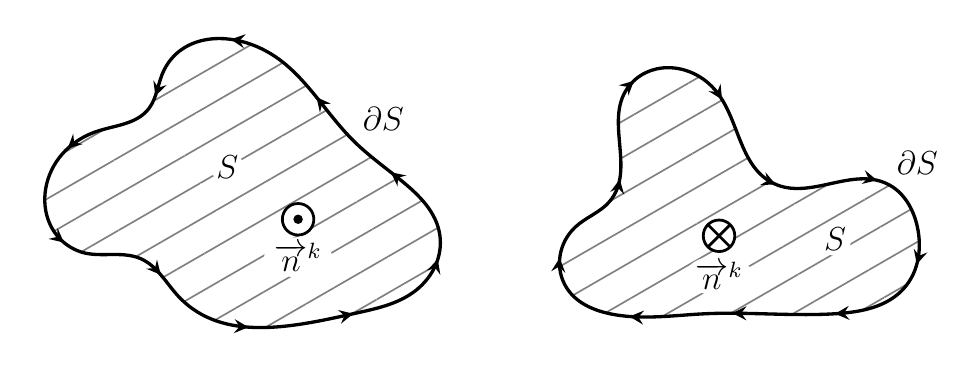
\begin{tikzpicture}[xshift=1.5cm]
\pgfmathsetmacro{\VectorDotRadius}{0.20}     % Radius of vector out/in
% define styles used in this picture
\tikzset{
BigTextFont/.style={font=\large},
every node/.style={font=\normalsize, text=black},
arrowstyle/.style={->, >=stealth}}

% vector in style
\tikzset{
       pics/.cd,
       vector in/.style 2 args={
       code={
       \fill[#1, white] (0,0) circle (#2); 
       \draw[#1] (0,0) circle (#2); % #2 is the radius
       \draw[#1] (45:#2) -- (225:#2) (135:#2) -- (315:#2); % Use #2 for line coordinates  
       }%end code   
       }%end style
}%end tikzset

% vector out style
\tikzset{
       pics/.cd,
       vector out/.style 2 args={
       code={
              \fill[#1, white] (0,0) circle (#2);
              \draw[#1] (0,0) circle (#2); % #2 is the radius
              \fill[#1] (0,0) circle (#2 * 0.3);
       }%end code   
       }%end style
}%end tikzset

% waypoint coordinates (in degrees, as seen from origin)
\begin{scope}[scale=1.0]
       \coordinate (BottomRight) at (1.2,0.0);     
       \coordinate (BottomRightStartCurve) at (2.0,0.3); 
       \coordinate (BottomRightEndCurve) at (2.3,1.0);
       \coordinate (MiddleRight) at (1.8,1.7);
       \coordinate (TopRight) at (1.2,2.2);
       \coordinate (TopMiddle) at (0.3,3.2);
       \coordinate (TopLeft) at (-1.2,3.1);
       \coordinate (MiddleLeft) at (-1.4,2.6);
       \coordinate (MiddleLeftStartBump) at (-2.1,2.3);
       \coordinate (BottomLeftEndBump) at (-2.3,0.8);
       \coordinate (BottomLeft) at (-1.5,0.7);
       \coordinate (BottomMiddle) at (-1.0,0.2);

       % pattern on area
       \fill[pattern={Lines[angle=30, distance=0.4cm, line width=0.6pt]}, pattern color=gray] (BottomRight) to[closed, curve through =
       {(BottomRightStartCurve) (BottomRightEndCurve) (MiddleRight) (TopRight) (TopMiddle) (TopLeft) (MiddleLeft) (MiddleLeftStartBump) (BottomLeftEndBump) (BottomLeft)}] (BottomMiddle);

       % drawing area
       \draw[postaction={decorate}, decoration={
              markings,
              mark = between positions 0.0 and 1 step 0.10 with {\arrow{stealth}},
              }]
       [very thick] (BottomRight) to[closed, curve through =
       {(BottomRightStartCurve) (BottomRightEndCurve) (MiddleRight) (TopRight) (TopMiddle) (TopLeft) (MiddleLeft) (MiddleLeftStartBump) (BottomLeftEndBump) (BottomLeft)}] (BottomMiddle);
       
       
       \node[BigTextFont, above right] at (TopRight) {$\partial S$};         % edge of S symbol
       \node[draw=white, ellipse, inner sep=0, fill=white, BigTextFont, above] at (-0.4, 1.65) {$S$};    % S symbol

       % Vector out symbol
       \coordinate (VectorOut) at (0.5,1.2);
       \path (VectorOut) pic {vector out={line width=1.0pt}{\VectorDotRadius}};
       \node[draw=white, ellipse, inner sep=0, fill=white, BigTextFont, below] at ($(VectorOut)-(0, \VectorDotRadius + 0.03)$) {$\overrightarrow{n}^k$}; 
\end{scope}


% CHECK
%plotting the waypoints
%\foreach \c in {(BottomRight), (BottomRightStartCurve), (BottomRightEndCurve), (MiddleRight),
% (TopRight), (TopMiddle), (TopLeft), (MiddleLeft), (MiddleLeftStartBump), (BottomLeftEndBump), (BottomLeft), (BottomMiddle)} \fill[red] \c circle (1.0mm);
\pgfmathsetmacro{\xshift}{6.0}
       % waypoint coordinates (in degrees, as seen from origin)
\begin{scope}[xshift=\xshift cm, scale=1.1]
       \coordinate (BottomRight) at (1.2,0.0);     
       \coordinate (BottomRightStartCurve) at (2.0,0.3); 
       \coordinate (BottomRightEndCurve) at (2.15,1.0);
       \coordinate (MiddleRight) at (1.8,1.5);
       \coordinate (TopRight) at (0.5,1.5);
       \coordinate (TopMiddle) at (-0.2,2.6);
       \coordinate (TopLeft) at (-1.2,2.6);
       \coordinate (MiddleLeft) at (-1.4,1.3);
       \coordinate (MiddleLeftStartBump) at (-1.8,1.0);
       \coordinate (BottomLeftEndBump) at (-1.9,0.3);
       \coordinate (BottomLeft) at (-1.4,0.0);
       \coordinate (BottomMiddle) at (-0.3,0.0);

       % pattern on area
       \fill[pattern={Lines[angle=30, distance=0.4cm, line width=0.6pt]}, pattern color=gray] (BottomRight) to[closed, curve through =
       {(BottomRightStartCurve) (BottomRightEndCurve) (MiddleRight) (TopRight) (TopMiddle) (TopLeft) (MiddleLeft) (MiddleLeftStartBump) (BottomLeftEndBump) (BottomLeft)}] (BottomMiddle);

       % drawing area
       \draw[postaction={decorate}, decoration={
              markings,
              mark = between positions 0.0 and 1 step 0.10 with {\arrowreversed{stealth}},
              }]
       [very thick] (BottomRight) to[closed, curve through =
       {(BottomRightStartCurve) (BottomRightEndCurve) (MiddleRight) (TopRight) (TopMiddle) (TopLeft) (MiddleLeft) (MiddleLeftStartBump) (BottomLeftEndBump) (BottomLeft)}] (BottomMiddle);

       \node[BigTextFont, above right] at (MiddleRight) {$\partial S$};
       \node[draw=white, ellipse, inner sep=0, fill=white, BigTextFont, above] at (1.2, 0.67) {$S$};
       %\path ($(-0.2, 1.3)+(\xshift,0)$) pic {vector in={line width=1.5pt}{\VectorDotRadius}}; 

       % Vector In symbol
       \coordinate (VectorIn) at (-0.14, 0.9);
       \path (VectorIn) pic {vector in={line width=1.0pt}{\VectorDotRadius}};
       \node[draw=white, ellipse, inner sep=0, fill=white, BigTextFont, below] at ($(VectorIn)-(0, \VectorDotRadius + 0.03)$) {$\overrightarrow{n}^k$}; 
\end{scope}

% CHECK
%plotting the waypoints
%\foreach \c in {(BottomRight), (BottomRightStartCurve), (BottomRightEndCurve), (MiddleRight),
%(TopRight), (TopMiddle), (TopLeft), (MiddleLeft), (MiddleLeftStartBump), (BottomLeftEndBump), (BottomLeft), (BottomMiddle)} \fill[red] \c circle (1.0mm);

\end{tikzpicture}

\end{document}